\documentclass[twoside]{book}

% Packages required by doxygen
\usepackage{fixltx2e}
\usepackage{calc}
\usepackage{doxygen}
\usepackage[export]{adjustbox} % also loads graphicx
\usepackage{graphicx}
\usepackage[utf8]{inputenc}
\usepackage{makeidx}
\usepackage{multicol}
\usepackage{multirow}
\PassOptionsToPackage{warn}{textcomp}
\usepackage{textcomp}
\usepackage[nointegrals]{wasysym}
\usepackage[table]{xcolor}

% Font selection
\usepackage[T1]{fontenc}
\usepackage[scaled=.90]{helvet}
\usepackage{courier}
\usepackage{amssymb}
\usepackage{sectsty}
\renewcommand{\familydefault}{\sfdefault}
\allsectionsfont{%
  \fontseries{bc}\selectfont%
  \color{darkgray}%
}
\renewcommand{\DoxyLabelFont}{%
  \fontseries{bc}\selectfont%
  \color{darkgray}%
}
\newcommand{\+}{\discretionary{\mbox{\scriptsize$\hookleftarrow$}}{}{}}

% Page & text layout
\usepackage{geometry}
\geometry{%
  a4paper,%
  top=2.5cm,%
  bottom=2.5cm,%
  left=2.5cm,%
  right=2.5cm%
}
\tolerance=750
\hfuzz=15pt
\hbadness=750
\setlength{\emergencystretch}{15pt}
\setlength{\parindent}{0cm}
\setlength{\parskip}{3ex plus 2ex minus 2ex}
\makeatletter
\renewcommand{\paragraph}{%
  \@startsection{paragraph}{4}{0ex}{-1.0ex}{1.0ex}{%
    \normalfont\normalsize\bfseries\SS@parafont%
  }%
}
\renewcommand{\subparagraph}{%
  \@startsection{subparagraph}{5}{0ex}{-1.0ex}{1.0ex}{%
    \normalfont\normalsize\bfseries\SS@subparafont%
  }%
}
\makeatother

% Headers & footers
\usepackage{fancyhdr}
\pagestyle{fancyplain}
\fancyhead[LE]{\fancyplain{}{\bfseries\thepage}}
\fancyhead[CE]{\fancyplain{}{}}
\fancyhead[RE]{\fancyplain{}{\bfseries\leftmark}}
\fancyhead[LO]{\fancyplain{}{\bfseries\rightmark}}
\fancyhead[CO]{\fancyplain{}{}}
\fancyhead[RO]{\fancyplain{}{\bfseries\thepage}}
\fancyfoot[LE]{\fancyplain{}{}}
\fancyfoot[CE]{\fancyplain{}{}}
\fancyfoot[RE]{\fancyplain{}{\bfseries\scriptsize Generated by Doxygen }}
\fancyfoot[LO]{\fancyplain{}{\bfseries\scriptsize Generated by Doxygen }}
\fancyfoot[CO]{\fancyplain{}{}}
\fancyfoot[RO]{\fancyplain{}{}}
\renewcommand{\footrulewidth}{0.4pt}
\renewcommand{\chaptermark}[1]{%
  \markboth{#1}{}%
}
\renewcommand{\sectionmark}[1]{%
  \markright{\thesection\ #1}%
}

% Indices & bibliography
\usepackage{natbib}
\usepackage[titles]{tocloft}
\setcounter{tocdepth}{3}
\setcounter{secnumdepth}{5}
\makeindex

% Hyperlinks (required, but should be loaded last)
\usepackage{ifpdf}
\ifpdf
  \usepackage[pdftex,pagebackref=true]{hyperref}
\else
  \usepackage[ps2pdf,pagebackref=true]{hyperref}
\fi
\hypersetup{%
  colorlinks=true,%
  linkcolor=blue,%
  citecolor=blue,%
  unicode%
}

% Custom commands
\newcommand{\clearemptydoublepage}{%
  \newpage{\pagestyle{empty}\cleardoublepage}%
}

\usepackage{caption}
\captionsetup{labelsep=space,justification=centering,font={bf},singlelinecheck=off,skip=4pt,position=top}

%===== C O N T E N T S =====

\begin{document}

% Titlepage & ToC
\hypersetup{pageanchor=false,
             bookmarksnumbered=true,
             pdfencoding=unicode
            }
\pagenumbering{roman}
\begin{titlepage}
\vspace*{7cm}
\begin{center}%
{\Large My Project }\\
\vspace*{1cm}
{\large Generated by Doxygen 1.8.11}\\
\end{center}
\end{titlepage}
\clearemptydoublepage
\tableofcontents
\clearemptydoublepage
\pagenumbering{arabic}
\hypersetup{pageanchor=true}

%--- Begin generated contents ---
\chapter{Lane Detection for Autonomous Vehicle}
\label{md_readme}
\hypertarget{md_readme}{}
\href{https://travis-ci.org/Indushekhar/AcmeLaneDetectionModule}{\tt } \href{https://coveralls.io/github/Indushekhar/AcmeLaneDetectionModule}{\tt } \href{https://opensource.org/licenses/MIT}{\tt }



 \subsection*{Overview}

The objective of this project was to design a lane detection (with lane turn signal and drive heading output) system for autonomous vehicles/\+Robots. The proposed lane detection algorithm by using a video feed input of a vehicle driving on the highway, detects the lane position and give drive heading angle. Which in turn can be passed to steering control system to move the vehicle inside the lane. Maintaining the lane on highway is very critical for autonomics vehicles. The system can be also be integrated with the popular Lane departure warning system designed to warn the driver when the vehicle begins to move out of its lane. The system being developed in C++ language provides very good real time performance.



\subsection*{Pipeline and Results}

The pipeline of the project can be summarized as \+:

\subsubsection*{1.\+Filter the Image}

First step is to remove the noise using median filter. This smooths the image and removes any undesired pixel values that could prevent the correct detection of the lanes

\subsubsection*{2.\+Apply edge detection to extract vertical edges}

Then apply edge detector to extract vertical edge. The intermediate output after edge detection is shown below



\subsubsection*{3.\+Extract the Region Of Interest}

As the image from previous step contains extra information which we do not need for lane finding, we extract the Region Of Interest.



\subsubsection*{4. Find lines using Hough Transform}

In this step we use Hough Transform to find lines on the image. Some paramter tuning is done to get peak hough lines.

\subsubsection*{5. Fit line}

In this step , we find out the peak hough lines, group them into two groups (positive, negative gradients) and extrapolate lines in each group. The lines are classified depending on the value of their slope and where their initial and final points are approximately located with respect to the center of the image.

\subsubsection*{6. Predict turn and Calculate drive head}

Using the intersection point of left and right lines, we get the vanishing point. Based on vanishing point and image center we predict the turns in the lane. For calculating drive head, coordinates of vanishing point in the image are used. Using simple trigonometry, atan2 is used to get angles in degree.

\subsubsection*{7. Plot the lane and drive head}



\subsubsection*{8. Results}

Output of the syste is quite good. The system was able to detect the lane even the part of the road which was whitish.



Output video can be seen at this \href{https://drive.google.com/drive/u/1/folders/1rqz6ssvReQMQbOU6W-9e-2ThTCKpCEad}{\tt link}

\subsection*{Dependencies}


\begin{DoxyEnumerate}
\item Open\+CV 3.\+3.\+0. or higher. This can be downloaded by following the steps of this \href{https://www.learnopencv.com/install-opencv3-on-ubuntu/}{\tt link}
\item For unit testing this project depends on gtest framework by Google.
\item C\+Make version at least 3.\+2.\+1
\end{DoxyEnumerate}

\subsection*{Standard install via command-\/line}


\begin{DoxyCode}
1 git clone --recursive https://github.com/Indushekhar/AcmeLaneDetectionModule
2 cd <path to repository>
3 mkdir build
4 cd build
5 cmake ..
6 make
\end{DoxyCode}
 \subsection*{Instructions to run the demo and tests}

Once the module is built correctly, to run the demo type the following command\+:


\begin{DoxyCode}
1 $ cd <build folder of the module>
2 $ ./app/main
\end{DoxyCode}


To run the unit tests, please execute the command given below\+:


\begin{DoxyCode}
1 $ ./test/system-test
\end{DoxyCode}


\subsection*{Dataset}

The dataset used for the system evaluation is taken from Advanced Lane Detection dataset from Udacity -\/ Self Driving Nanodegree program. The dataset can be downloaded from the link below \+:

\href{https://drive.google.com/drive/folders/1XR0v4H73xvUQDT92OO_ud9MVqnTNOXJO?usp=sharing}{\tt https\+://drive.\+google.\+com/drive/folders/1\+X\+R0v4\+H73xv\+U\+Q\+D\+T92\+O\+O\+\_\+ud9\+M\+Vqn\+T\+N\+O\+X\+J\+O?usp=sharing}

\subsection*{Solo Iterative Process and Sprint Planning}

Sprint planning details can be found on the following link.

\href{https://docs.google.com/document/d/1Fxr27H92AX2Sr3t2H6NpyOqamlBIBs7oRIrZiXUN6i0/edit?usp=sharing}{\tt https\+://docs.\+google.\+com/document/d/1\+Fxr27\+H92\+A\+X2\+Sr3t2\+H6\+Npy\+Oqaml\+B\+I\+Bs7o\+R\+Ir\+Zi\+X\+U\+N6i0/edit?usp=sharing}

The software is being be developed by following the Solo Iterative Process(\+S\+I\+P). A product backlog, release backlog and work log(time log and code defect log) is being used as structure of the whole project. The log can be viewed at following link \+:

\href{https://docs.google.com/spreadsheets/d/1IO5K6LXyBzSSsjxovvstrDoHjlVawQgHOqON_L0iJLY/edit?usp=sharing}{\tt https\+://docs.\+google.\+com/spreadsheets/d/1\+I\+O5\+K6\+L\+Xy\+Bz\+S\+Ssjxovvstr\+Do\+Hjl\+Vaw\+Qg\+H\+Oq\+O\+N\+\_\+\+L0i\+J\+L\+Y/edit?usp=sharing}

\subsection*{Doumentation}

The douments for this project is already present in docs folder.

To generate documentation install dependencies first


\begin{DoxyCode}
1 $ sudo apt-get install doxygen
2 $ sudo apt-get install doxygen-gui
3 $ doxywizard
\end{DoxyCode}
 It will open gui version. On the top of the gui window, It will require a working directory. Set the directory. Give the source folder path as the repository folder and check the recursive checkbox. Give target directory where you want to save the documentations files.

\subsection*{License}

M\+IT License

Copyright (c) 2018 Indushekhar Singh

Permission is hereby granted, free of charge, to any person obtaining a copy of this software and associated documentation files (the \char`\"{}\+Software\char`\"{}), to deal in the Software without restriction, including without limitation the rights to use, copy, modify, merge, publish, distribute, sublicense, and/or sell copies of the Software, and to permit persons to whom the Software is furnished to do so, subject to the following conditions\+:

The above copyright notice and this permission notice shall be included in all copies or substantial portions of the Software.

T\+HE S\+O\+F\+T\+W\+A\+RE IS P\+R\+O\+V\+I\+D\+ED \char`\"{}\+A\+S I\+S\char`\"{}, W\+I\+T\+H\+O\+UT W\+A\+R\+R\+A\+N\+TY OF A\+NY K\+I\+ND, E\+X\+P\+R\+E\+SS OR I\+M\+P\+L\+I\+ED, I\+N\+C\+L\+U\+D\+I\+NG B\+UT N\+OT L\+I\+M\+I\+T\+ED TO T\+HE W\+A\+R\+R\+A\+N\+T\+I\+ES OF M\+E\+R\+C\+H\+A\+N\+T\+A\+B\+I\+L\+I\+TY, F\+I\+T\+N\+E\+SS F\+OR A P\+A\+R\+T\+I\+C\+U\+L\+AR P\+U\+R\+P\+O\+SE A\+ND N\+O\+N\+I\+N\+F\+R\+I\+N\+G\+E\+M\+E\+NT. IN NO E\+V\+E\+NT S\+H\+A\+LL T\+HE A\+U\+T\+H\+O\+RS OR C\+O\+P\+Y\+R\+I\+G\+HT H\+O\+L\+D\+E\+RS BE L\+I\+A\+B\+LE F\+OR A\+NY C\+L\+A\+IM, D\+A\+M\+A\+G\+ES OR O\+T\+H\+ER L\+I\+A\+B\+I\+L\+I\+TY, W\+H\+E\+T\+H\+ER IN AN A\+C\+T\+I\+ON OF C\+O\+N\+T\+R\+A\+CT, T\+O\+RT OR O\+T\+H\+E\+R\+W\+I\+SE, A\+R\+I\+S\+I\+NG F\+R\+OM, O\+UT OF OR IN C\+O\+N\+N\+E\+C\+T\+I\+ON W\+I\+TH T\+HE S\+O\+F\+T\+W\+A\+RE OR T\+HE U\+SE OR O\+T\+H\+ER D\+E\+A\+L\+I\+N\+GS IN T\+HE S\+O\+F\+T\+W\+A\+RE. 
\chapter{Class Index}
\section{Class List}
Here are the classes, structs, unions and interfaces with brief descriptions\+:\begin{DoxyCompactList}
\item\contentsline{section}{\hyperlink{class_lane_detection}{Lane\+Detection} \\*Class for \hyperlink{class_lane_detection}{Lane\+Detection} }{\pageref{class_lane_detection}}{}
\item\contentsline{section}{\hyperlink{class_plot_manager}{Plot\+Manager} \\*Class for \hyperlink{class_plot_manager}{Plot\+Manager} }{\pageref{class_plot_manager}}{}
\item\contentsline{section}{\hyperlink{class_system_manager}{System\+Manager} \\*Class for \hyperlink{class_lane_detection}{Lane\+Detection} }{\pageref{class_system_manager}}{}
\end{DoxyCompactList}

\chapter{File Index}
\section{File List}
Here is a list of all documented files with brief descriptions\+:\begin{DoxyCompactList}
\item\contentsline{section}{app/\hyperlink{_lane_detection_8cpp}{Lane\+Detection.\+cpp} \\*\hyperlink{class_lane_detection}{Lane\+Detection} class }{\pageref{_lane_detection_8cpp}}{}
\item\contentsline{section}{app/\hyperlink{main_8cpp}{main.\+cpp} \\*Main script }{\pageref{main_8cpp}}{}
\item\contentsline{section}{app/\hyperlink{_plot_manager_8cpp}{Plot\+Manager.\+cpp} \\*\hyperlink{class_plot_manager}{Plot\+Manager} class }{\pageref{_plot_manager_8cpp}}{}
\item\contentsline{section}{app/\hyperlink{_system_manager_8cpp}{System\+Manager.\+cpp} \\*\hyperlink{class_system_manager}{System\+Manager} class }{\pageref{_system_manager_8cpp}}{}
\item\contentsline{section}{include/\hyperlink{_lane_detection_8hpp}{Lane\+Detection.\+hpp} \\*\hyperlink{class_lane_detection}{Lane\+Detection} class }{\pageref{_lane_detection_8hpp}}{}
\item\contentsline{section}{include/\hyperlink{_plot_manager_8hpp}{Plot\+Manager.\+hpp} \\*\hyperlink{class_plot_manager}{Plot\+Manager} class }{\pageref{_plot_manager_8hpp}}{}
\item\contentsline{section}{include/\hyperlink{_system_manager_8hpp}{System\+Manager.\+hpp} \\*\hyperlink{class_system_manager}{System\+Manager} class }{\pageref{_system_manager_8hpp}}{}
\end{DoxyCompactList}

\chapter{Class Documentation}
\hypertarget{class_lane_detection}{}\section{Lane\+Detection Class Reference}
\label{class_lane_detection}\index{Lane\+Detection@{Lane\+Detection}}


Class for \hyperlink{class_lane_detection}{Lane\+Detection}.  




{\ttfamily \#include $<$Lane\+Detection.\+hpp$>$}

\subsection*{Public Member Functions}
\begin{DoxyCompactItemize}
\item 
\hyperlink{class_lane_detection_a731f54ebd16a6ad77ff51e413415d1d9}{Lane\+Detection} ()
\begin{DoxyCompactList}\small\item\em Constructor to initialize the object. \end{DoxyCompactList}\item 
\hyperlink{class_lane_detection_afdccabf18bc0137fafb973624e8c3df3}{$\sim$\+Lane\+Detection} ()\hypertarget{class_lane_detection_afdccabf18bc0137fafb973624e8c3df3}{}\label{class_lane_detection_afdccabf18bc0137fafb973624e8c3df3}

\begin{DoxyCompactList}\small\item\em Destroys the object. \end{DoxyCompactList}\item 
cv\+::\+Mat \hyperlink{class_lane_detection_a7c7413cec74ede4469eb090133887f9d}{filter} (cv\+::\+Mat input\+\_\+image)
\begin{DoxyCompactList}\small\item\em Method to do image filtering. \end{DoxyCompactList}\item 
cv\+::\+Mat \hyperlink{class_lane_detection_a89874335db28ff99b4b117dc4e21792f}{edge\+Detector} (cv\+::\+Mat image\+\_\+filter)
\begin{DoxyCompactList}\small\item\em Method to do edge detection. \end{DoxyCompactList}\item 
cv\+::\+Mat \hyperlink{class_lane_detection_af720e7949d6863e9d3e2100fc2655ce4}{roi\+Extract} (cv\+::\+Mat image\+\_\+edge)
\begin{DoxyCompactList}\small\item\em Method to do extract region of interest. \end{DoxyCompactList}\item 
std\+::vector$<$ cv\+::\+Vec4i $>$ \hyperlink{class_lane_detection_a3d2a00fcb2a6487d6cbd16c72768c4e4}{get\+Lines} (cv\+::\+Mat image\+\_\+roi)
\begin{DoxyCompactList}\small\item\em Method to do find line in the image. \end{DoxyCompactList}\item 
std\+::vector$<$ cv\+::\+Point $>$ \hyperlink{class_lane_detection_a58b5c9a016cbdad5fc2698492d157085}{line\+Fitting} (std\+::vector$<$ cv\+::\+Vec4i $>$ lines, cv\+::\+Mat input\+\_\+image)
\begin{DoxyCompactList}\small\item\em Method to do fit a single line in the image. \end{DoxyCompactList}\item 
std\+::string \hyperlink{class_lane_detection_ab3b0a639451e5056ff2d62d8ebd06fc9}{turn\+Prediction} (double thresh\+\_\+vanish)
\begin{DoxyCompactList}\small\item\em Method to predict turn. \end{DoxyCompactList}\item 
double \hyperlink{class_lane_detection_abd0c50facc187e7dc6c09c5325a5f013}{drive\+Heading} ()
\begin{DoxyCompactList}\small\item\em Method to calculate drive heading. \end{DoxyCompactList}\end{DoxyCompactItemize}


\subsection{Detailed Description}
Class for \hyperlink{class_lane_detection}{Lane\+Detection}. 

\subsection{Constructor \& Destructor Documentation}
\index{Lane\+Detection@{Lane\+Detection}!Lane\+Detection@{Lane\+Detection}}
\index{Lane\+Detection@{Lane\+Detection}!Lane\+Detection@{Lane\+Detection}}
\subsubsection[{\texorpdfstring{Lane\+Detection()}{LaneDetection()}}]{\setlength{\rightskip}{0pt plus 5cm}Lane\+Detection\+::\+Lane\+Detection (
\begin{DoxyParamCaption}
{}
\end{DoxyParamCaption}
)}\hypertarget{class_lane_detection_a731f54ebd16a6ad77ff51e413415d1d9}{}\label{class_lane_detection_a731f54ebd16a6ad77ff51e413415d1d9}


Constructor to initialize the object. 

Constructs the object. 

\subsection{Member Function Documentation}
\index{Lane\+Detection@{Lane\+Detection}!drive\+Heading@{drive\+Heading}}
\index{drive\+Heading@{drive\+Heading}!Lane\+Detection@{Lane\+Detection}}
\subsubsection[{\texorpdfstring{drive\+Heading()}{driveHeading()}}]{\setlength{\rightskip}{0pt plus 5cm}double Lane\+Detection\+::drive\+Heading (
\begin{DoxyParamCaption}
{}
\end{DoxyParamCaption}
)}\hypertarget{class_lane_detection_abd0c50facc187e7dc6c09c5325a5f013}{}\label{class_lane_detection_abd0c50facc187e7dc6c09c5325a5f013}


Method to calculate drive heading. 

Calculate the drive heading.


\begin{DoxyParams}{Parameters}
{\em None} & \\
\hline
\end{DoxyParams}
\begin{DoxyReturn}{Returns}
None 
\end{DoxyReturn}
\index{Lane\+Detection@{Lane\+Detection}!edge\+Detector@{edge\+Detector}}
\index{edge\+Detector@{edge\+Detector}!Lane\+Detection@{Lane\+Detection}}
\subsubsection[{\texorpdfstring{edge\+Detector(cv\+::\+Mat image\+\_\+filter)}{edgeDetector(cv::Mat image_filter)}}]{\setlength{\rightskip}{0pt plus 5cm}cv\+::\+Mat Lane\+Detection\+::edge\+Detector (
\begin{DoxyParamCaption}
\item[{cv\+::\+Mat}]{image\+\_\+filter}
\end{DoxyParamCaption}
)}\hypertarget{class_lane_detection_a89874335db28ff99b4b117dc4e21792f}{}\label{class_lane_detection_a89874335db28ff99b4b117dc4e21792f}


Method to do edge detection. 

Do edge detection on filtered image.


\begin{DoxyParams}{Parameters}
{\em input\+\_\+filter} & Input image frame \\
\hline
\end{DoxyParams}
\begin{DoxyReturn}{Returns}
Image with edge detected 
\end{DoxyReturn}
\index{Lane\+Detection@{Lane\+Detection}!filter@{filter}}
\index{filter@{filter}!Lane\+Detection@{Lane\+Detection}}
\subsubsection[{\texorpdfstring{filter(cv\+::\+Mat input\+\_\+image)}{filter(cv::Mat input_image)}}]{\setlength{\rightskip}{0pt plus 5cm}cv\+::\+Mat Lane\+Detection\+::filter (
\begin{DoxyParamCaption}
\item[{cv\+::\+Mat}]{input\+\_\+image}
\end{DoxyParamCaption}
)}\hypertarget{class_lane_detection_a7c7413cec74ede4469eb090133887f9d}{}\label{class_lane_detection_a7c7413cec74ede4469eb090133887f9d}


Method to do image filtering. 

Do image filtering on input image.


\begin{DoxyParams}{Parameters}
{\em input\+\_\+image} & Input image frame to be filtered \\
\hline
\end{DoxyParams}
\begin{DoxyReturn}{Returns}
Filtered Image 
\end{DoxyReturn}
\index{Lane\+Detection@{Lane\+Detection}!get\+Lines@{get\+Lines}}
\index{get\+Lines@{get\+Lines}!Lane\+Detection@{Lane\+Detection}}
\subsubsection[{\texorpdfstring{get\+Lines(cv\+::\+Mat image\+\_\+roi)}{getLines(cv::Mat image_roi)}}]{\setlength{\rightskip}{0pt plus 5cm}std\+::vector$<$ cv\+::\+Vec4i $>$ Lane\+Detection\+::get\+Lines (
\begin{DoxyParamCaption}
\item[{cv\+::\+Mat}]{image\+\_\+roi}
\end{DoxyParamCaption}
)}\hypertarget{class_lane_detection_a3d2a00fcb2a6487d6cbd16c72768c4e4}{}\label{class_lane_detection_a3d2a00fcb2a6487d6cbd16c72768c4e4}


Method to do find line in the image. 

Find lines on the image.


\begin{DoxyParams}{Parameters}
{\em input\+\_\+roi} & Input image with region of interest \\
\hline
\end{DoxyParams}
\begin{DoxyReturn}{Returns}
detected line 
\end{DoxyReturn}
\index{Lane\+Detection@{Lane\+Detection}!line\+Fitting@{line\+Fitting}}
\index{line\+Fitting@{line\+Fitting}!Lane\+Detection@{Lane\+Detection}}
\subsubsection[{\texorpdfstring{line\+Fitting(std\+::vector$<$ cv\+::\+Vec4i $>$ lines, cv\+::\+Mat input\+\_\+image)}{lineFitting(std::vector< cv::Vec4i > lines, cv::Mat input_image)}}]{\setlength{\rightskip}{0pt plus 5cm}std\+::vector$<$ cv\+::\+Point $>$ Lane\+Detection\+::line\+Fitting (
\begin{DoxyParamCaption}
\item[{std\+::vector$<$ cv\+::\+Vec4i $>$}]{lines, }
\item[{cv\+::\+Mat}]{image\+\_\+edge}
\end{DoxyParamCaption}
)}\hypertarget{class_lane_detection_a58b5c9a016cbdad5fc2698492d157085}{}\label{class_lane_detection_a58b5c9a016cbdad5fc2698492d157085}


Method to do fit a single line in the image. 

Do the line fitting.


\begin{DoxyParams}{Parameters}
{\em input\+\_\+roi} & Input image with region of interest \\
\hline
\end{DoxyParams}
\begin{DoxyReturn}{Returns}
detected line 
\end{DoxyReturn}
\index{Lane\+Detection@{Lane\+Detection}!roi\+Extract@{roi\+Extract}}
\index{roi\+Extract@{roi\+Extract}!Lane\+Detection@{Lane\+Detection}}
\subsubsection[{\texorpdfstring{roi\+Extract(cv\+::\+Mat image\+\_\+edge)}{roiExtract(cv::Mat image_edge)}}]{\setlength{\rightskip}{0pt plus 5cm}cv\+::\+Mat Lane\+Detection\+::roi\+Extract (
\begin{DoxyParamCaption}
\item[{cv\+::\+Mat}]{image\+\_\+edge}
\end{DoxyParamCaption}
)}\hypertarget{class_lane_detection_af720e7949d6863e9d3e2100fc2655ce4}{}\label{class_lane_detection_af720e7949d6863e9d3e2100fc2655ce4}


Method to do extract region of interest. 

Extract region of interest.


\begin{DoxyParams}{Parameters}
{\em input\+\_\+edge} & Input image with edge detected \\
\hline
\end{DoxyParams}
\begin{DoxyReturn}{Returns}
Image with region of interest 
\end{DoxyReturn}
\index{Lane\+Detection@{Lane\+Detection}!turn\+Prediction@{turn\+Prediction}}
\index{turn\+Prediction@{turn\+Prediction}!Lane\+Detection@{Lane\+Detection}}
\subsubsection[{\texorpdfstring{turn\+Prediction(double thresh\+\_\+vanish)}{turnPrediction(double thresh_vanish)}}]{\setlength{\rightskip}{0pt plus 5cm}std\+::string Lane\+Detection\+::turn\+Prediction (
\begin{DoxyParamCaption}
\item[{double}]{thresh\+\_\+vanish}
\end{DoxyParamCaption}
)}\hypertarget{class_lane_detection_ab3b0a639451e5056ff2d62d8ebd06fc9}{}\label{class_lane_detection_ab3b0a639451e5056ff2d62d8ebd06fc9}


Method to predict turn. 

Predict the turn.


\begin{DoxyParams}{Parameters}
{\em thresh\+\_\+vanish} & Threshhold for deciding vanishing point \\
\hline
\end{DoxyParams}
\begin{DoxyReturn}{Returns}
turn prediction \+: left, right or straight turn 
\end{DoxyReturn}


The documentation for this class was generated from the following files\+:\begin{DoxyCompactItemize}
\item 
include/\hyperlink{_lane_detection_8hpp}{Lane\+Detection.\+hpp}\item 
app/\hyperlink{_lane_detection_8cpp}{Lane\+Detection.\+cpp}\end{DoxyCompactItemize}

\hypertarget{class_plot_manager}{}\section{Plot\+Manager Class Reference}
\label{class_plot_manager}\index{Plot\+Manager@{Plot\+Manager}}


Class for \hyperlink{class_plot_manager}{Plot\+Manager}.  




{\ttfamily \#include $<$Plot\+Manager.\+hpp$>$}

\subsection*{Public Member Functions}
\begin{DoxyCompactItemize}
\item 
\hyperlink{class_plot_manager_a9a7b472058d22e8bbf7712686b998aae}{Plot\+Manager} ()
\begin{DoxyCompactList}\small\item\em Constructs the object. \end{DoxyCompactList}\item 
\hyperlink{class_plot_manager_ab5b318f61ab5e2c50d0bf7d09a05c331}{$\sim$\+Plot\+Manager} ()
\begin{DoxyCompactList}\small\item\em Constructs the object. \end{DoxyCompactList}\item 
void \hyperlink{class_plot_manager_a314f6e531f88366eb71c40eb84140c3e}{plot} (cv\+::\+Mat input\+\_\+image, std\+::vector$<$ cv\+::\+Point $>$ line\+\_\+fit, std\+::string turn\+Direction, double drive\+\_\+heading, bool show\+\_\+plot)
\begin{DoxyCompactList}\small\item\em Method to plot the lane and drive heading on input image. \end{DoxyCompactList}\end{DoxyCompactItemize}


\subsection{Detailed Description}
Class for \hyperlink{class_plot_manager}{Plot\+Manager}. 

\subsection{Constructor \& Destructor Documentation}
\index{Plot\+Manager@{Plot\+Manager}!Plot\+Manager@{Plot\+Manager}}
\index{Plot\+Manager@{Plot\+Manager}!Plot\+Manager@{Plot\+Manager}}
\subsubsection[{\texorpdfstring{Plot\+Manager()}{PlotManager()}}]{\setlength{\rightskip}{0pt plus 5cm}Plot\+Manager\+::\+Plot\+Manager (
\begin{DoxyParamCaption}
{}
\end{DoxyParamCaption}
)}\hypertarget{class_plot_manager_a9a7b472058d22e8bbf7712686b998aae}{}\label{class_plot_manager_a9a7b472058d22e8bbf7712686b998aae}


Constructs the object. 

Constructor to initialize \index{Plot\+Manager@{Plot\+Manager}!````~Plot\+Manager@{$\sim$\+Plot\+Manager}}
\index{````~Plot\+Manager@{$\sim$\+Plot\+Manager}!Plot\+Manager@{Plot\+Manager}}
\subsubsection[{\texorpdfstring{$\sim$\+Plot\+Manager()}{~PlotManager()}}]{\setlength{\rightskip}{0pt plus 5cm}Plot\+Manager\+::$\sim$\+Plot\+Manager (
\begin{DoxyParamCaption}
{}
\end{DoxyParamCaption}
)}\hypertarget{class_plot_manager_ab5b318f61ab5e2c50d0bf7d09a05c331}{}\label{class_plot_manager_ab5b318f61ab5e2c50d0bf7d09a05c331}


Constructs the object. 

Destructor 

\subsection{Member Function Documentation}
\index{Plot\+Manager@{Plot\+Manager}!plot@{plot}}
\index{plot@{plot}!Plot\+Manager@{Plot\+Manager}}
\subsubsection[{\texorpdfstring{plot(cv\+::\+Mat input\+\_\+image, std\+::vector$<$ cv\+::\+Point $>$ line\+\_\+fit, std\+::string turn\+Direction, double drive\+\_\+heading, bool show\+\_\+plot)}{plot(cv::Mat input_image, std::vector< cv::Point > line_fit, std::string turnDirection, double drive_heading, bool show_plot)}}]{\setlength{\rightskip}{0pt plus 5cm}void Plot\+Manager\+::plot (
\begin{DoxyParamCaption}
\item[{cv\+::\+Mat}]{input\+Image, }
\item[{std\+::vector$<$ cv\+::\+Point $>$}]{lane, }
\item[{std\+::string}]{turn, }
\item[{double}]{drive\+\_\+heading, }
\item[{bool}]{show\+\_\+plot}
\end{DoxyParamCaption}
)}\hypertarget{class_plot_manager_a314f6e531f88366eb71c40eb84140c3e}{}\label{class_plot_manager_a314f6e531f88366eb71c40eb84140c3e}


Method to plot the lane and drive heading on input image. 

Plot the lane and drive heading on input image.


\begin{DoxyParams}{Parameters}
{\em input\+\_\+image} & Input image \\
\hline
{\em line\+\_\+fit} & Both lane which are to be plotted \\
\hline
{\em turn\+Direction} & Turn direction left, right or straight \\
\hline
{\em drive\+\_\+heading} & Drive heading value \\
\hline
{\em show\+\_\+plot} & whether to show plot or not\\
\hline
{\em input\+\_\+image} & Input image \\
\hline
{\em line\+\_\+fit} & Both lane which are to be plotted \\
\hline
{\em turn\+Direction} & Turn direction left, right or straight \\
\hline
{\em drive\+\_\+heading} & Drive heading value \\
\hline
{\em show\+\_\+plot} & whether to show plot or not \\
\hline
\end{DoxyParams}
\begin{DoxyReturn}{Returns}
None 
\end{DoxyReturn}


The documentation for this class was generated from the following files\+:\begin{DoxyCompactItemize}
\item 
include/\hyperlink{_plot_manager_8hpp}{Plot\+Manager.\+hpp}\item 
app/\hyperlink{_plot_manager_8cpp}{Plot\+Manager.\+cpp}\end{DoxyCompactItemize}

\hypertarget{class_system_manager}{}\section{System\+Manager Class Reference}
\label{class_system_manager}\index{System\+Manager@{System\+Manager}}


Class for \hyperlink{class_lane_detection}{Lane\+Detection}.  




{\ttfamily \#include $<$System\+Manager.\+hpp$>$}

\subsection*{Public Member Functions}
\begin{DoxyCompactItemize}
\item 
\hyperlink{class_system_manager_a2f8a3e2e1929be50ef8702629f50bb94}{System\+Manager} ()
\begin{DoxyCompactList}\small\item\em Constructor to initialize the object. \end{DoxyCompactList}\item 
\hyperlink{class_system_manager_a0fa2e3c0906401494f6bf4e482aecc0d}{$\sim$\+System\+Manager} ()\hypertarget{class_system_manager_a0fa2e3c0906401494f6bf4e482aecc0d}{}\label{class_system_manager_a0fa2e3c0906401494f6bf4e482aecc0d}

\begin{DoxyCompactList}\small\item\em Destroys the object. \end{DoxyCompactList}\item 
int \hyperlink{class_system_manager_ae189ebfcc72d8fb1e67ddf7215bdc77a}{run\+Lane} (std\+::string filename, int no\+\_\+of\+\_\+frames, bool show\+\_\+plot)
\begin{DoxyCompactList}\small\item\em Method for running the whole \hyperlink{class_lane_detection}{Lane\+Detection} system. \end{DoxyCompactList}\end{DoxyCompactItemize}


\subsection{Detailed Description}
Class for \hyperlink{class_lane_detection}{Lane\+Detection}. 

\subsection{Constructor \& Destructor Documentation}
\index{System\+Manager@{System\+Manager}!System\+Manager@{System\+Manager}}
\index{System\+Manager@{System\+Manager}!System\+Manager@{System\+Manager}}
\subsubsection[{\texorpdfstring{System\+Manager()}{SystemManager()}}]{\setlength{\rightskip}{0pt plus 5cm}System\+Manager\+::\+System\+Manager (
\begin{DoxyParamCaption}
{}
\end{DoxyParamCaption}
)}\hypertarget{class_system_manager_a2f8a3e2e1929be50ef8702629f50bb94}{}\label{class_system_manager_a2f8a3e2e1929be50ef8702629f50bb94}


Constructor to initialize the object. 

Constructs the object. 

\subsection{Member Function Documentation}
\index{System\+Manager@{System\+Manager}!run\+Lane@{run\+Lane}}
\index{run\+Lane@{run\+Lane}!System\+Manager@{System\+Manager}}
\subsubsection[{\texorpdfstring{run\+Lane(std\+::string filename, int no\+\_\+of\+\_\+frames, bool show\+\_\+plot)}{runLane(std::string filename, int no_of_frames, bool show_plot)}}]{\setlength{\rightskip}{0pt plus 5cm}int System\+Manager\+::run\+Lane (
\begin{DoxyParamCaption}
\item[{std\+::string}]{filename, }
\item[{int}]{no\+\_\+of\+\_\+frames, }
\item[{bool}]{show\+\_\+plot}
\end{DoxyParamCaption}
)}\hypertarget{class_system_manager_ae189ebfcc72d8fb1e67ddf7215bdc77a}{}\label{class_system_manager_ae189ebfcc72d8fb1e67ddf7215bdc77a}


Method for running the whole \hyperlink{class_lane_detection}{Lane\+Detection} system. 

run the complete lane detection system


\begin{DoxyParams}{Parameters}
{\em filename} & Path to the input video to be tested \\
\hline
{\em no\+\_\+of\+\_\+frames} & Number of frames to be processed \\
\hline
{\em show\+\_\+plot} & Whether to show the frames or not \\
\hline
\end{DoxyParams}


The documentation for this class was generated from the following files\+:\begin{DoxyCompactItemize}
\item 
include/\hyperlink{_system_manager_8hpp}{System\+Manager.\+hpp}\item 
app/\hyperlink{_system_manager_8cpp}{System\+Manager.\+cpp}\end{DoxyCompactItemize}

\chapter{File Documentation}
\hypertarget{_lane_detection_8cpp}{}\section{app/\+Lane\+Detection.cpp File Reference}
\label{_lane_detection_8cpp}\index{app/\+Lane\+Detection.\+cpp@{app/\+Lane\+Detection.\+cpp}}


\hyperlink{class_lane_detection}{Lane\+Detection} class.  


{\ttfamily \#include $<$math.\+h$>$}\\*
{\ttfamily \#include $<$string$>$}\\*
{\ttfamily \#include $<$vector$>$}\\*
{\ttfamily \#include \char`\"{}../include/\+Lane\+Detection.\+hpp\char`\"{}}\\*
Include dependency graph for Lane\+Detection.\+cpp\+:
\nopagebreak
\begin{figure}[H]
\begin{center}
\leavevmode
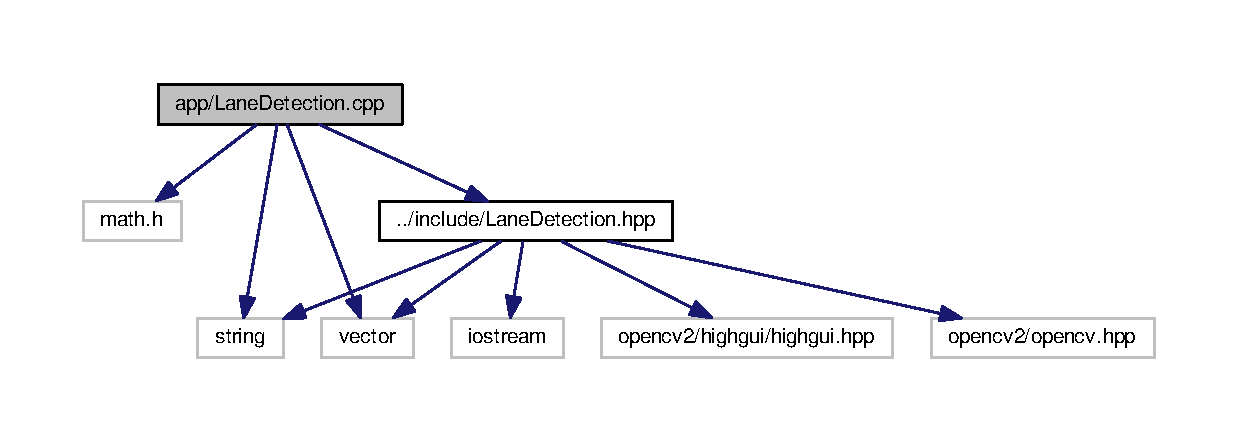
\includegraphics[width=350pt]{_lane_detection_8cpp__incl}
\end{center}
\end{figure}
\subsection*{Macros}
\begin{DoxyCompactItemize}
\item 
\#define {\bfseries PI}~3.\+14159265\hypertarget{_lane_detection_8cpp_a598a3330b3c21701223ee0ca14316eca}{}\label{_lane_detection_8cpp_a598a3330b3c21701223ee0ca14316eca}

\end{DoxyCompactItemize}


\subsection{Detailed Description}
\hyperlink{class_lane_detection}{Lane\+Detection} class. 

Implementation of \hyperlink{class_lane_detection}{Lane\+Detection} class for detecting lanes \begin{DoxyAuthor}{Author}
Indushekhar Singh 
\end{DoxyAuthor}
\begin{DoxyVersion}{Version}
1.\+0 
\end{DoxyVersion}
\begin{DoxyCopyright}{Copyright}
M\+IT License (c) 2018 Indushekhar Singh 
\end{DoxyCopyright}

\hypertarget{main_8cpp}{}\section{app/main.cpp File Reference}
\label{main_8cpp}\index{app/main.\+cpp@{app/main.\+cpp}}


main script  


{\ttfamily \#include $<$iostream$>$}\\*
{\ttfamily \#include $<$string$>$}\\*
{\ttfamily \#include $<$vector$>$}\\*
{\ttfamily \#include \char`\"{}../include/\+System\+Manager.\+hpp\char`\"{}}\\*
Include dependency graph for main.\+cpp\+:
\nopagebreak
\begin{figure}[H]
\begin{center}
\leavevmode
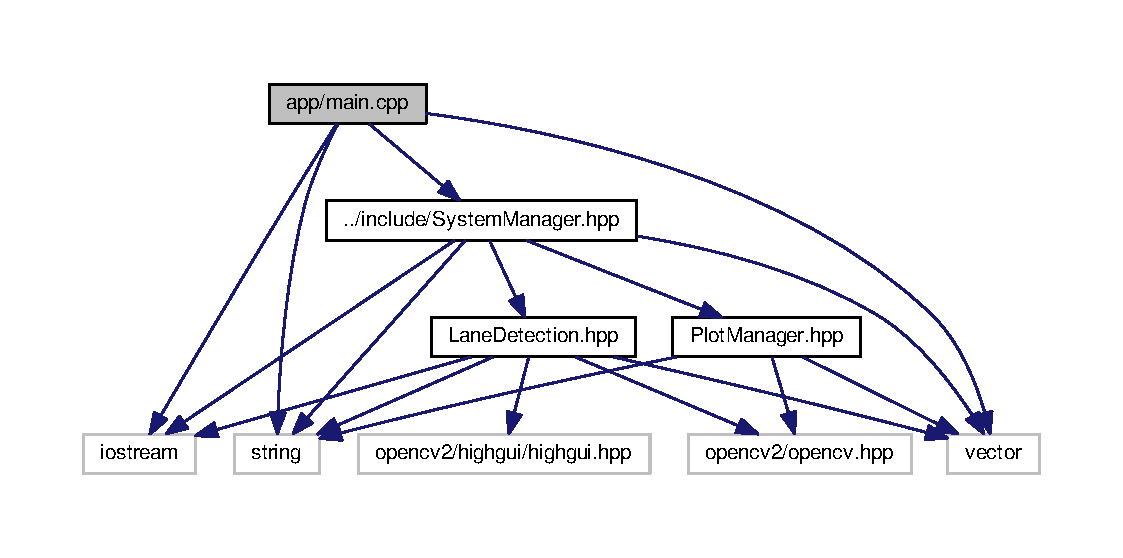
\includegraphics[width=350pt]{main_8cpp__incl}
\end{center}
\end{figure}
\subsection*{Functions}
\begin{DoxyCompactItemize}
\item 
int {\bfseries main} ()\hypertarget{main_8cpp_ae66f6b31b5ad750f1fe042a706a4e3d4}{}\label{main_8cpp_ae66f6b31b5ad750f1fe042a706a4e3d4}

\end{DoxyCompactItemize}


\subsection{Detailed Description}
main script 

Used to run the system \begin{DoxyAuthor}{Author}
Indushekhar Singh 
\end{DoxyAuthor}
\begin{DoxyVersion}{Version}
1.\+0 
\end{DoxyVersion}
\begin{DoxyCopyright}{Copyright}
M\+IT License (c) 2018 Indushekhar Singh 
\end{DoxyCopyright}

\hypertarget{_plot_manager_8cpp}{}\section{app/\+Plot\+Manager.cpp File Reference}
\label{_plot_manager_8cpp}\index{app/\+Plot\+Manager.\+cpp@{app/\+Plot\+Manager.\+cpp}}


\hyperlink{class_plot_manager}{Plot\+Manager} class.  


{\ttfamily \#include $<$string$>$}\\*
{\ttfamily \#include $<$vector$>$}\\*
{\ttfamily \#include $<$iostream$>$}\\*
{\ttfamily \#include \char`\"{}opencv2/opencv.\+hpp\char`\"{}}\\*
{\ttfamily \#include \char`\"{}../include/\+Plot\+Manager.\+hpp\char`\"{}}\\*
Include dependency graph for Plot\+Manager.\+cpp\+:
\nopagebreak
\begin{figure}[H]
\begin{center}
\leavevmode
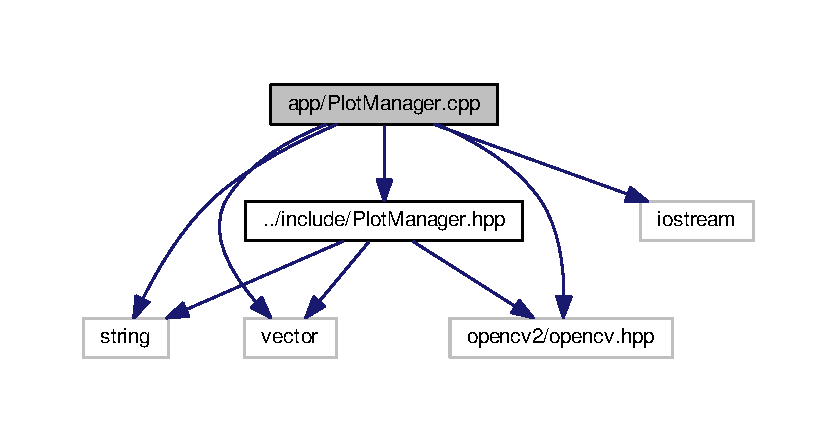
\includegraphics[width=350pt]{_plot_manager_8cpp__incl}
\end{center}
\end{figure}


\subsection{Detailed Description}
\hyperlink{class_plot_manager}{Plot\+Manager} class. 

Implementation of \hyperlink{class_plot_manager}{Plot\+Manager} class \begin{DoxyAuthor}{Author}
Indushekhar Singh 
\end{DoxyAuthor}
\begin{DoxyVersion}{Version}
1.\+0 
\end{DoxyVersion}
\begin{DoxyCopyright}{Copyright}
M\+IT License (c) 2018 Indushekhar Singh 
\end{DoxyCopyright}

\hypertarget{_system_manager_8cpp}{}\section{app/\+System\+Manager.cpp File Reference}
\label{_system_manager_8cpp}\index{app/\+System\+Manager.\+cpp@{app/\+System\+Manager.\+cpp}}


\hyperlink{class_system_manager}{System\+Manager} class.  


{\ttfamily \#include $<$string$>$}\\*
{\ttfamily \#include $<$vector$>$}\\*
{\ttfamily \#include \char`\"{}../include/\+System\+Manager.\+hpp\char`\"{}}\\*
{\ttfamily \#include $<$opencv2/highgui/highgui.\+hpp$>$}\\*
Include dependency graph for System\+Manager.\+cpp\+:
\nopagebreak
\begin{figure}[H]
\begin{center}
\leavevmode
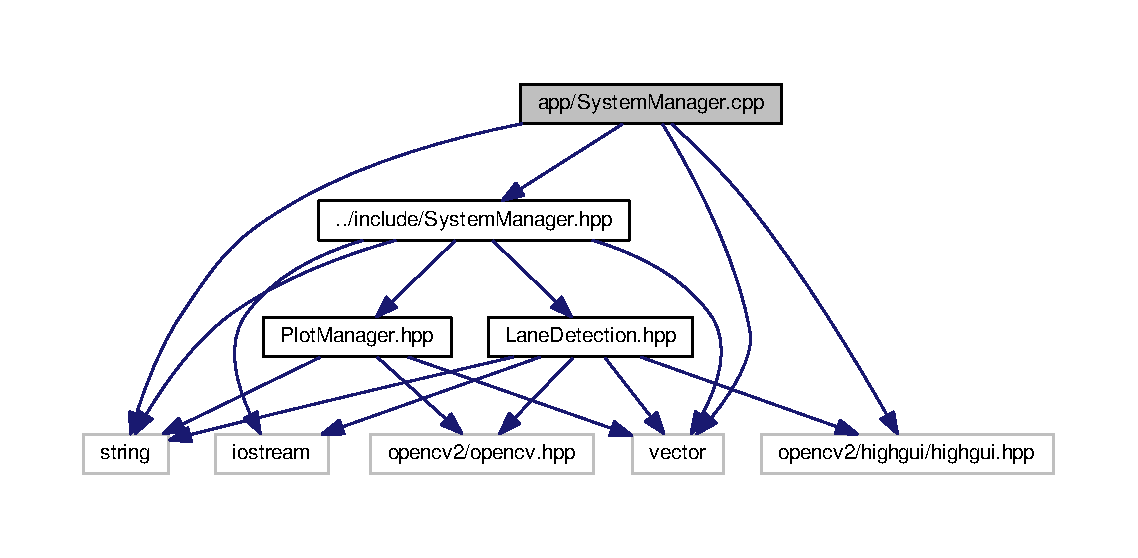
\includegraphics[width=350pt]{_system_manager_8cpp__incl}
\end{center}
\end{figure}


\subsection{Detailed Description}
\hyperlink{class_system_manager}{System\+Manager} class. 

Implementation of \hyperlink{class_system_manager}{System\+Manager} class \begin{DoxyAuthor}{Author}
Indushekhar Singh 
\end{DoxyAuthor}
\begin{DoxyVersion}{Version}
1.\+0 
\end{DoxyVersion}
\begin{DoxyCopyright}{Copyright}
M\+IT License (c) 2018 Indushekhar Singh 
\end{DoxyCopyright}

\hypertarget{_lane_detection_8hpp}{}\section{include/\+Lane\+Detection.hpp File Reference}
\label{_lane_detection_8hpp}\index{include/\+Lane\+Detection.\+hpp@{include/\+Lane\+Detection.\+hpp}}


\hyperlink{class_lane_detection}{Lane\+Detection} class.  


{\ttfamily \#include $<$iostream$>$}\\*
{\ttfamily \#include $<$string$>$}\\*
{\ttfamily \#include $<$vector$>$}\\*
{\ttfamily \#include $<$opencv2/highgui/highgui.\+hpp$>$}\\*
{\ttfamily \#include \char`\"{}opencv2/opencv.\+hpp\char`\"{}}\\*
Include dependency graph for Lane\+Detection.\+hpp\+:
\nopagebreak
\begin{figure}[H]
\begin{center}
\leavevmode
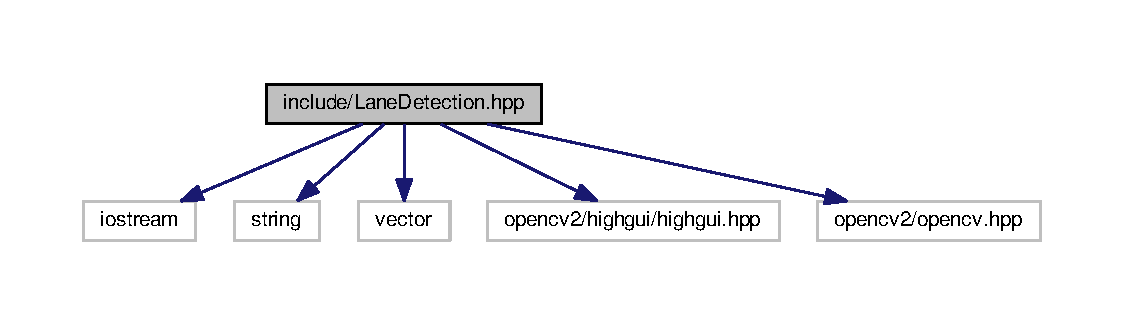
\includegraphics[width=350pt]{_lane_detection_8hpp__incl}
\end{center}
\end{figure}
This graph shows which files directly or indirectly include this file\+:
\nopagebreak
\begin{figure}[H]
\begin{center}
\leavevmode
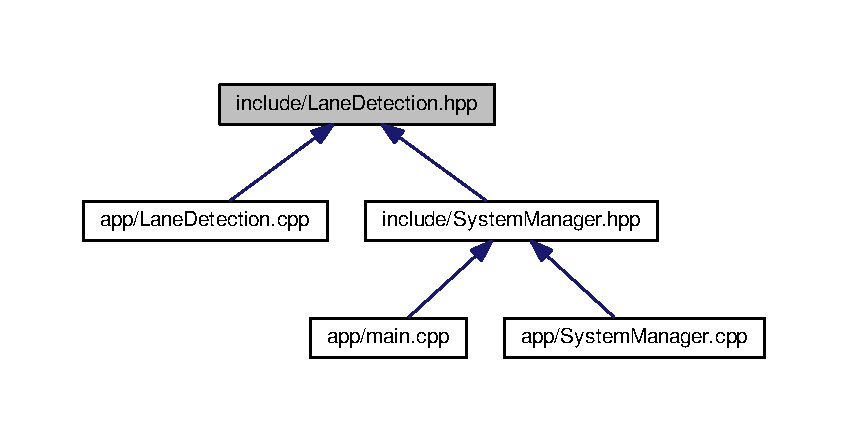
\includegraphics[width=350pt]{_lane_detection_8hpp__dep__incl}
\end{center}
\end{figure}
\subsection*{Classes}
\begin{DoxyCompactItemize}
\item 
class \hyperlink{class_lane_detection}{Lane\+Detection}
\begin{DoxyCompactList}\small\item\em Class for \hyperlink{class_lane_detection}{Lane\+Detection}. \end{DoxyCompactList}\end{DoxyCompactItemize}


\subsection{Detailed Description}
\hyperlink{class_lane_detection}{Lane\+Detection} class. 

Definition of \hyperlink{class_lane_detection}{Lane\+Detection} class \begin{DoxyAuthor}{Author}
Indushekhar Singh 
\end{DoxyAuthor}
\begin{DoxyVersion}{Version}
1.\+0 
\end{DoxyVersion}
\begin{DoxyCopyright}{Copyright}
M\+IT License (c) 2018 Indushekhar Singh 
\end{DoxyCopyright}

\hypertarget{_plot_manager_8hpp}{}\section{include/\+Plot\+Manager.hpp File Reference}
\label{_plot_manager_8hpp}\index{include/\+Plot\+Manager.\+hpp@{include/\+Plot\+Manager.\+hpp}}


\hyperlink{class_plot_manager}{Plot\+Manager} class.  


{\ttfamily \#include $<$string$>$}\\*
{\ttfamily \#include $<$vector$>$}\\*
{\ttfamily \#include \char`\"{}opencv2/opencv.\+hpp\char`\"{}}\\*
Include dependency graph for Plot\+Manager.\+hpp\+:
\nopagebreak
\begin{figure}[H]
\begin{center}
\leavevmode
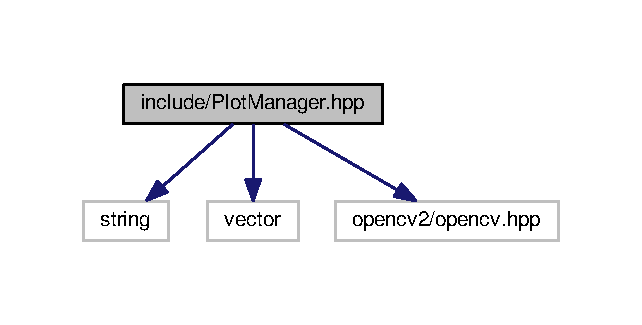
\includegraphics[width=308pt]{_plot_manager_8hpp__incl}
\end{center}
\end{figure}
This graph shows which files directly or indirectly include this file\+:
\nopagebreak
\begin{figure}[H]
\begin{center}
\leavevmode
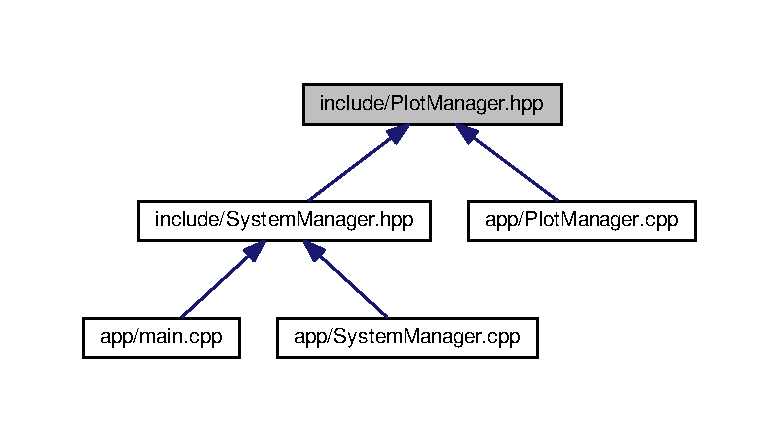
\includegraphics[width=350pt]{_plot_manager_8hpp__dep__incl}
\end{center}
\end{figure}
\subsection*{Classes}
\begin{DoxyCompactItemize}
\item 
class \hyperlink{class_plot_manager}{Plot\+Manager}
\begin{DoxyCompactList}\small\item\em Class for \hyperlink{class_plot_manager}{Plot\+Manager}. \end{DoxyCompactList}\end{DoxyCompactItemize}


\subsection{Detailed Description}
\hyperlink{class_plot_manager}{Plot\+Manager} class. 

Definition of \hyperlink{class_plot_manager}{Plot\+Manager} class \begin{DoxyAuthor}{Author}
Indushekhar Singh 
\end{DoxyAuthor}
\begin{DoxyVersion}{Version}
1.\+0 
\end{DoxyVersion}
\begin{DoxyCopyright}{Copyright}
M\+IT License (c) 2018 Indushekhar Singh 
\end{DoxyCopyright}

\hypertarget{_system_manager_8hpp}{}\section{include/\+System\+Manager.hpp File Reference}
\label{_system_manager_8hpp}\index{include/\+System\+Manager.\+hpp@{include/\+System\+Manager.\+hpp}}


\hyperlink{class_system_manager}{System\+Manager} class.  


{\ttfamily \#include $<$iostream$>$}\\*
{\ttfamily \#include $<$vector$>$}\\*
{\ttfamily \#include $<$string$>$}\\*
{\ttfamily \#include \char`\"{}Lane\+Detection.\+hpp\char`\"{}}\\*
{\ttfamily \#include \char`\"{}Plot\+Manager.\+hpp\char`\"{}}\\*
Include dependency graph for System\+Manager.\+hpp\+:
\nopagebreak
\begin{figure}[H]
\begin{center}
\leavevmode
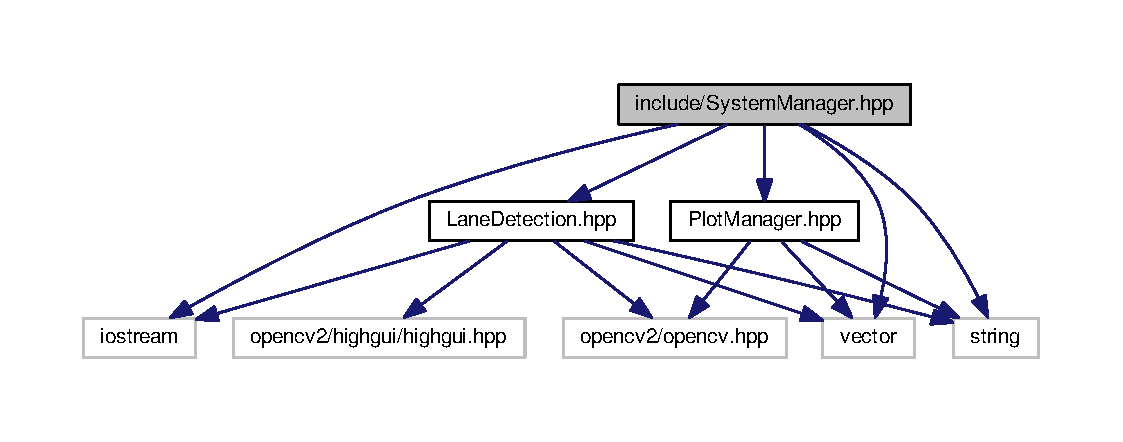
\includegraphics[width=350pt]{_system_manager_8hpp__incl}
\end{center}
\end{figure}
This graph shows which files directly or indirectly include this file\+:
\nopagebreak
\begin{figure}[H]
\begin{center}
\leavevmode
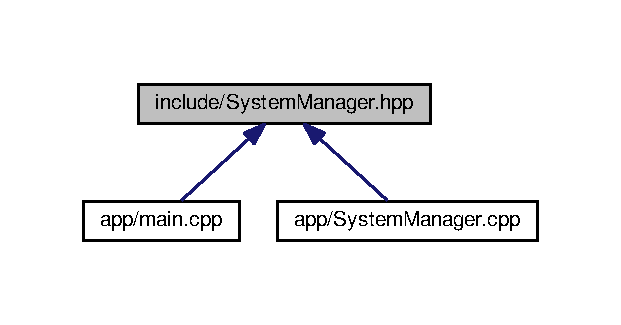
\includegraphics[width=298pt]{_system_manager_8hpp__dep__incl}
\end{center}
\end{figure}
\subsection*{Classes}
\begin{DoxyCompactItemize}
\item 
class \hyperlink{class_system_manager}{System\+Manager}
\begin{DoxyCompactList}\small\item\em Class for \hyperlink{class_lane_detection}{Lane\+Detection}. \end{DoxyCompactList}\end{DoxyCompactItemize}


\subsection{Detailed Description}
\hyperlink{class_system_manager}{System\+Manager} class. 

Definition of \hyperlink{class_system_manager}{System\+Manager} class \begin{DoxyAuthor}{Author}
Indushekhar Singh 
\end{DoxyAuthor}
\begin{DoxyVersion}{Version}
1.\+0 
\end{DoxyVersion}
\begin{DoxyCopyright}{Copyright}
M\+IT License (c) 2018 Indushekhar Singh 
\end{DoxyCopyright}

%--- End generated contents ---

% Index
\backmatter
\newpage
\phantomsection
\clearemptydoublepage
\addcontentsline{toc}{chapter}{Index}
\printindex

\end{document}
